\documentclass[a4paper,12pt]{report}            % [forma A4, taille police] {Type}
\usepackage[utf8]{inputenc}                
\usepackage[T1]{fontenc}                        % Codage des fontes TeX
\usepackage[francais]{babel}
\usepackage{graphicx}
\usepackage{wrapfig}
\usepackage{fancyhdr}
\usepackage{xcolor}
\usepackage{hyperref}
\usepackage{listings}
\usepackage{fullpage}
\usepackage{eso-pic}
\usepackage{titlesec}
\titleformat{\chapter}[hang]{\bf\huge}{\thechapter}{2pc}{}
\lstset {numbers=left ,stepnumber=1,firstnumber=0,numberfirstline=true}
\hypersetup{
    bookmarks=true,         % show bookmarks bar?
    unicode=false,          % non-Latin characters in Acrobat’s bookmarks
    pdftoolbar=true,        % show Acrobat’s toolbar?
    pdfmenubar=true,        % show Acrobat’s menu?
    pdffitwindow=false,     % window fit to page when opened
    pdfstartview={FitH},    % fits the width of the page to the window
    pdftitle={My title},    % title
    pdfauthor={Author},     % author
    pdfsubject={Subject},   % subject of the document
    pdfcreator={Creator},   % creator of the document
    pdfproducer={Producer}, % producer of the document
    pdfkeywords={keyword1, key2, key3}, % list of keywords
    pdfnewwindow=true,      % links in new PDF window
    colorlinks=true,       % false: boxed links; true: colored links
    linkcolor=black,          % color of internal links (change box color with linkbordercolor)
    citecolor=green,        % color of links to bibliography
    filecolor=magenta,      % color of file links
    urlcolor=blue           % color of external links
}

\author{Samuel HUET \& Thomas COUTANT}
\title{\huge{Le Mixer}}

\begin{document}
\maketitle
\renewcommand{\contentsname}{SOMMAIRE} % Dans le corps du document,avant la commande \tableofcontents.
\tableofcontents

\chapter{Le mélangeur à diode}
\addcontentsline{toc}{chapter}{Le mélangeur à diode}

\section{Principe de fonctionnement}
    Un mélangeur permet de transposer un signal radio (RF) par soustraction ou addition avec
une autre fréquence venant d'un oscillateur local (OL). Nous obtenons donc en sortie des
signaux (FI) aux fréquences $FI = |OL - RF|$ ou $FI = |OL + RF|$\\
    Le mélangeur à diodes utilise l'équation liant tension/courant non linéaire
des diodes afin de réalise le mélange. Il est consitué de 4 diodes et de deux transformateurs.
Bien que le mélangeur à diode génère moins moins de signaux indésirables que certains autres montages,
il s'agit d'une structure passive, qui assure une perte d'un moins 6dB sur sa sortie.\\
\begin{center}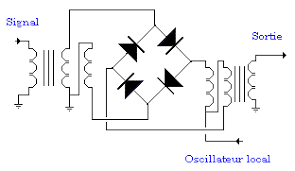
\includegraphics[scale = 1]{pic/schema_mixer.png}\\ \end{center}

    La non linéarité des diodes implique inévitablement des signaux parasites sur la sortie,
pouvant s'écrire : $Vs = a + b(Ve) + c(Ve)^{2} + d(Ve)^{3} ...$\\
    Pour des signaux d'entrée dont l'excursion est faible, la  droite de charge de la diode peut 
être aproximé à une droite, mais les signaux dont l'excursion est plus large implique des signaux parasites.\\
    Voici le schema du melangeur. Nous pouvons y voir les fréquences d'entré $F_{RF}$, $F_{OL}$ ainsi que la
fréquence de sortie $F_{IF}$ expliqués plus haut. Celui que nous allons utiliser pour ce TP est le ZFM-2 de Mini Circuits.\\
\begin{center}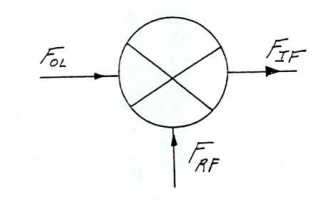
\includegraphics[scale = 0.4]{pic/mixer_logo.png}\\ \end{center}

\section{Spectre théorique}

\begin{center}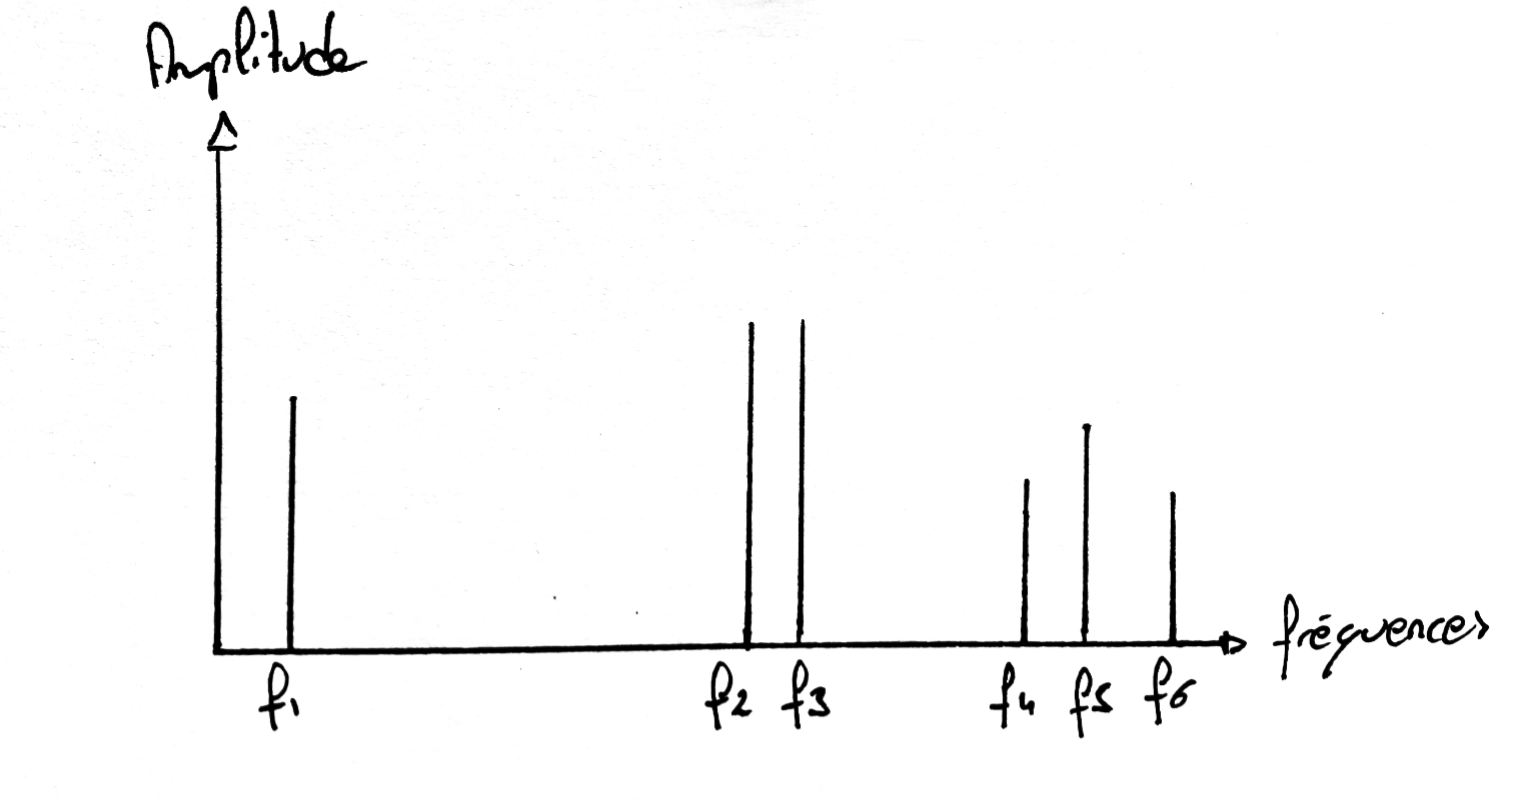
\includegraphics[scale = 0.25]{pic/Spectre_theorique.png}\\ \end{center}

où : 
\begin{itemize}
    \item $f_{1} = |OL-RF|$
    \item $f_{2} = OL$ 
    \item $f_{3} = RF$
    \item $f_{4} = 2OL$
    \item $f_{5} = |OL+RF|$
    \item $f_{6} = 2RF$
\end{itemize}


\bigskip
Dans la pratique, nous pouvons dors et déjà supposer que le spectre sera beaucoup
plus fournis de part de nombreuses fréquences parasites non prises en compte.

\chapter{Mise en situation}
\addcontentsline{toc}{chapter}{Mise en situation}
\section{Cablage}

Avant de cabler notre mixer, et afin de s'assurer de la précision de la mesure, 
nous pouvant effectuer un petit test au sujet des pertes du aux cables et aux connecteur.
Pour cela, nous branchons un oscillateur à un analyseur de spectre comme ceci :\\
\begin{center}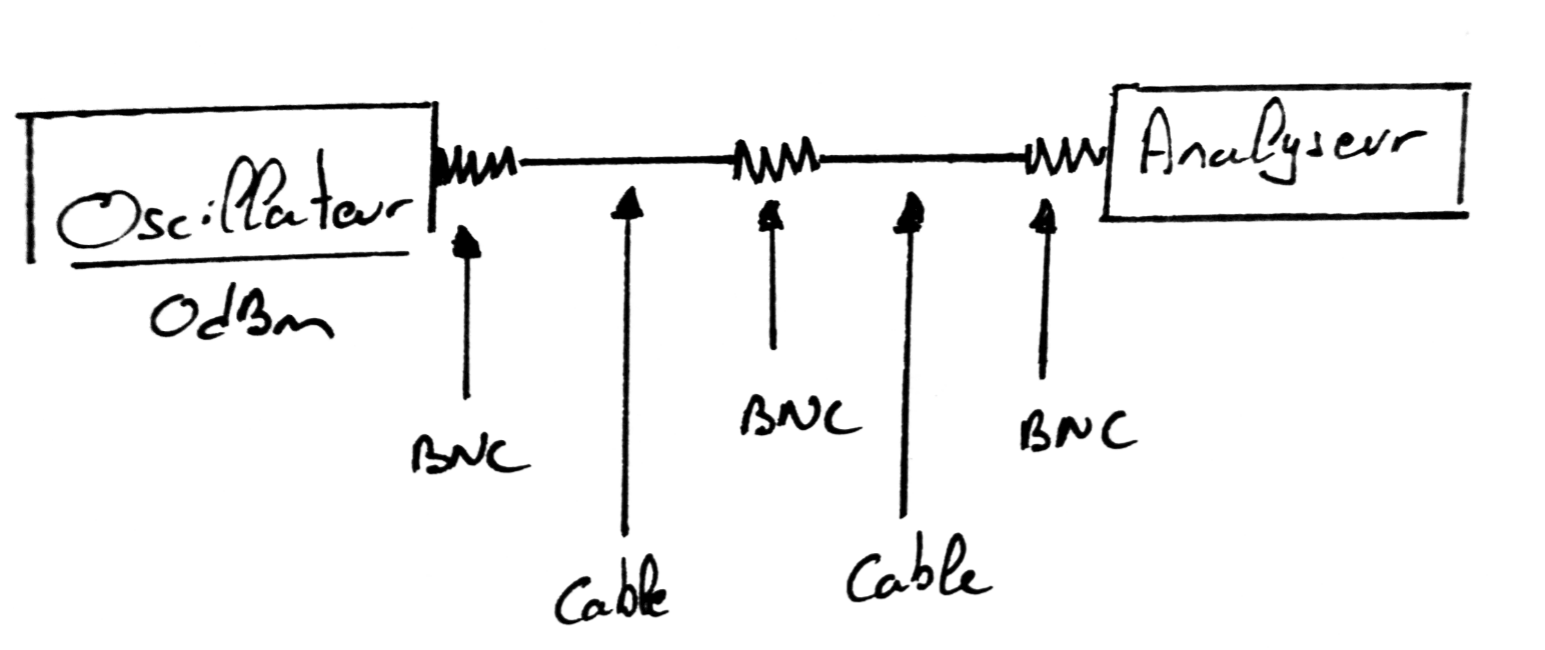
\includegraphics[scale = 0.2]{pic/mesure_perte.png}\\ \end{center}

    Ainsi, les pertes du aux coax sont bien visible sur l'analyseur de spectre. On suppose
la perte du au connecteur du milieu négligeable. D'après cette experience, les pertes sont de
0.14 dB. Pour la précision des mesures, il faudra alors ajouter 0.14 à toutes ces dernières.


    Maintenant que nous avons déterminer les pertes, nous pouvons brancher notre mixer
comme ceci :
\begin{center}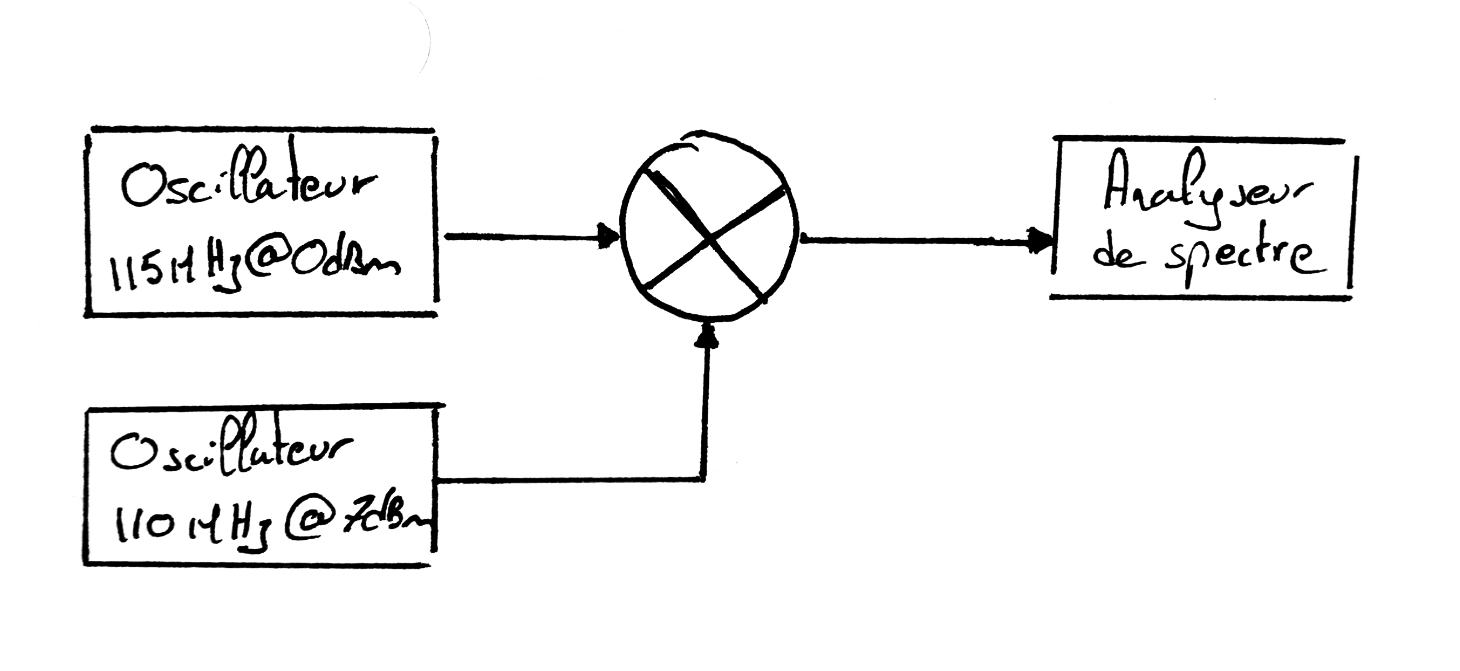
\includegraphics[scale = 0.2]{pic/cablage.png}\\ \end{center}


    L'analyse des fréquences et de leur puissances respective nous donne le spectre suivant.
Sur ce spectre, le 0dBm de l'amplitude relative correspond en réalité à -47dBm absolue. Nous 
pouvons constatier que les deux raies principales attentures sont bel et bien présentes :
à savoir $|OL+RF| = 225 MHz \mbox{ et } |OL-RF| = 5 MHz$. Cependant, nous pouvons constater 
beaucoup plus de bruit qu'attendu sur le spectre théorique.
\begin{center}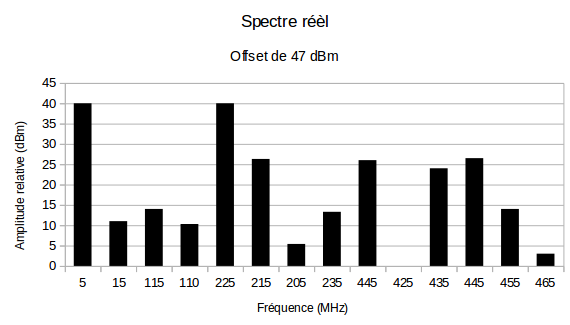
\includegraphics[scale = 0.7]{pic/spectre_reel.png}\i\ \end{center}


    Bien sur nous retrouvons également les fréquences énoncés plus haut dans la partie théorique.
avec :
\begin{itemize}
    \item $f_{RF} = 115 MHz$
    \item $f_{OL} = 110 MHz$ 
    \item $f_{|OL-RF|} = 5 MHz$
    \item $f_{|OL+RF|} = 225 MHz$
    \item $f_{2OL} = 220 MHz$
    \item $f_{2RF} = 230 MHz$
\end{itemize}
Et parmis les fréquences non prises en compte dans le spectre théorique, on retrouve :
\begin{itemize}
    \item $f_{|2(RF-OL)-(RF+OL)|} = 215 MHz$
    \item $f_{|2(OL+RF)-(RF-OL)|} = 445 MHz$ 
\end{itemize}

\chapter{Mesures caractéristiques}
\addcontentsline{toc}{chapter}{Mesure caractéristiques}
\section{Perte de conversion}
    La perte de conversion est une caractéristique intrasec du composant. Cette mesure
corespond au nombre de dB perdu lorsque le signal d'entré traverse le composant.
Sur un mixer, le signal entrant est donc le signal radio et le signal sortant est la
fréquence image.  
\begin{center}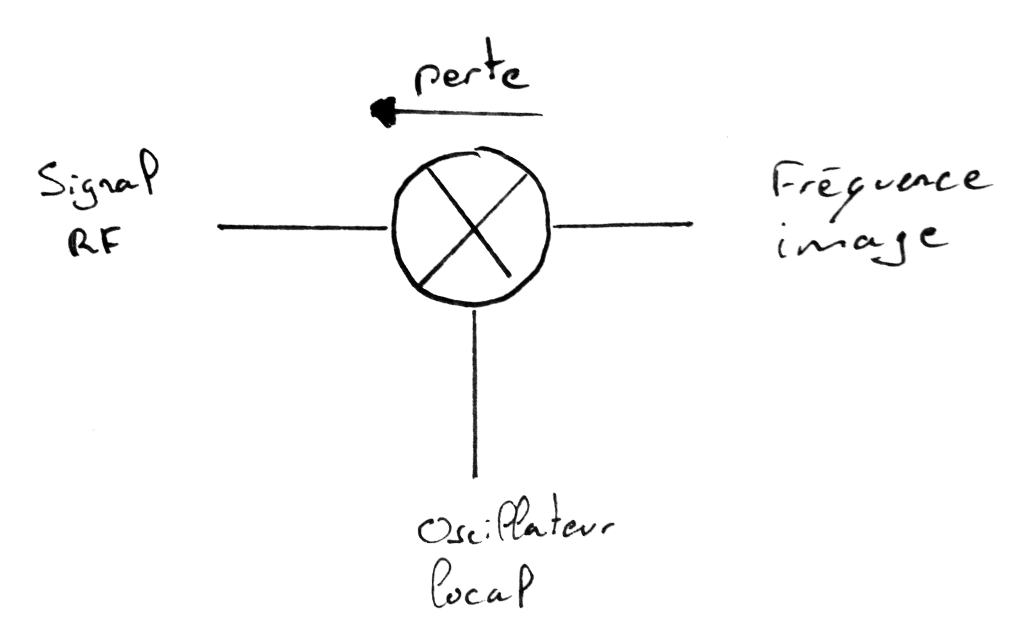
\includegraphics[scale = 0.3]{pic/perte_conversion.png}\\ \end{center}
Nous avons donc injecté un signal en entré, en regardant la sortie à l'analyseur de spectre
et sans oublier de prendre en compte les pertes du aux cables,
nous pouvons en déduire les pertes de conversion. \\
En utilisant les données fournis par les mesures précédentes, nous avons donc en entré 0dBm, 
et en sortie -7 dBm, auquel nous pouvons ajouter 0.14. Ce qui nous donne une
sortie à -6.86 dBm.
$$ \mbox{Perte par conversion }= 6.86 dB$$


\newpage
\section{Isolation}

    L'isolation représente la capacité qu'a un signal entrant, à se retrouver sur d'autre
broches du composant. Concernant le mixer, il existe deux isolations mesurables : 
\begin{itemize}
    \item L'isolation entre RF et OL
    \item L'isolation entre OL et FI
\end{itemize}
Bien sur, plus l'isolation est haute, meilleur est le composant.
\begin{center}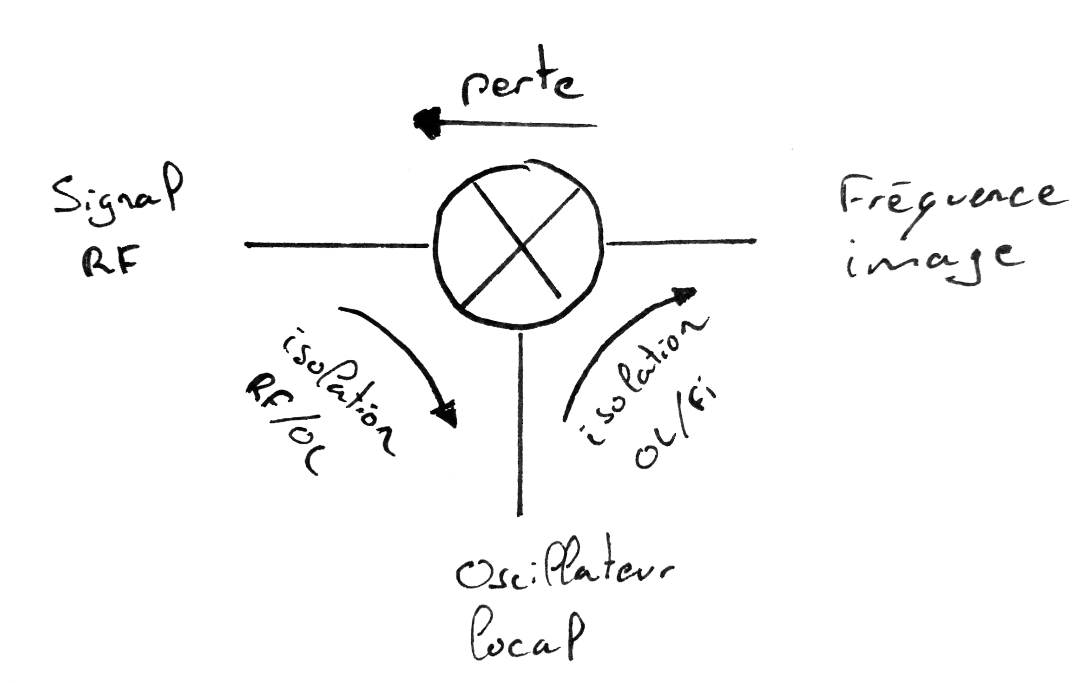
\includegraphics[scale = 0.3]{pic/isolation.png}\\ \end{center}

    Pour mesurer l'isolation RF/OL, nous branchons simplement la broche RF sur un oscillateur, 
puis la broche OL sur l'analyseur de spectre. Il ne faut pas oublier de charger (50$\Omega$) sans
quoi la mesure sera faussé.\\
Donc en prenant en compte la perte du aux cables :\\
$$Isolation_{RF/OL} = -50dB$$
Ce qui correspond à la courbe représenté sur la datasheet (pour un signal de 115 MHZ)
    Pour mesurer l'isolation OL/RF, il suffit de brancher la broche OL sur l'oscillateur, 
puis la sortie du mixer sur l'analyseur de spectre. Nous n'oublions pas de chercher la
broche RF.
$$Isolation_{OL/FI} = -31dB$$

    Bien sur ces valeurs sont à prendre pour les fréquences utilisé et varient plus ou moins
selon ce paramètre. \\
\begin{center}
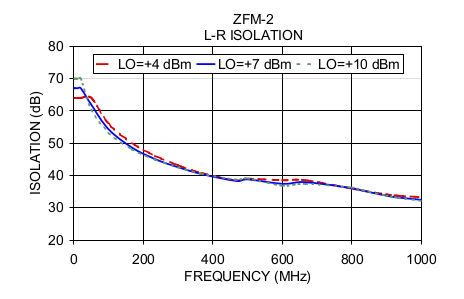
\includegraphics[scale = 0.45]{pic/isolation1_datasheet.png}
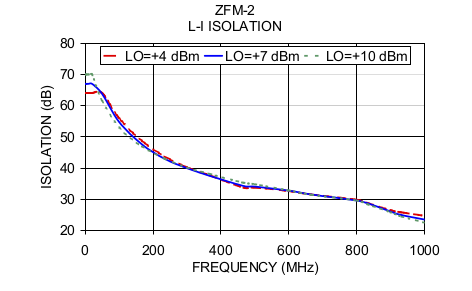
\includegraphics[scale = 0.45]{pic/isolation2_datasheet.png}
\end{center}

\section{Point de compression}
Les amplificateurs sont sujets à des phénomènes de saturation en puissance sur leur sortie
C'est à dire que pour de fortes puissances en entrée l'amplificateur perdra toute sa linéarité
Le point de compression à 1 dB permet de caractériser la limite du fonctionnement linéaire de l'amplificateur. 
Pour cela on changera la puissance d'entré (RF) en la plaçant à une valeur assez basse, nous sommme partie de 
-15dBm dans notre cas. Et l'on observe la puissance en sortie sur l'analyseur de spectre, en se plaçant sur la raie OL-RF ou OL+RF.
Ainsi nous avons procédé à un relevé balayant la puissance de -15dBm à 1dB en observant à chaque crant la sortie.
Ce qui nous a permis d'obtenir cette courbes:
\begin{center}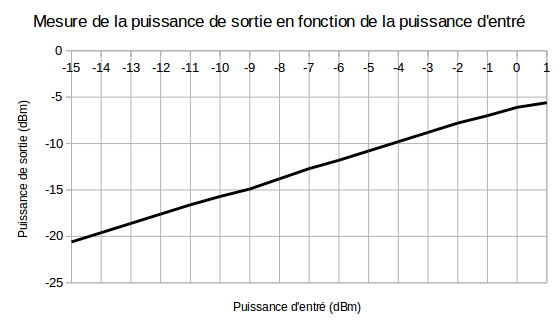
\includegraphics[scale = 0.7]{pic/graph_pout.png}\\ \end{center}
Le cablage est le même que lors de la phase de test on opère juste un changement sur le synthétiseur de la fréquence RF.
Grâce à la courbes que nous avons déterminé, nous pouvoir alors voir que le point de compression se trouve pour 1dBm en entré.
\section{IP3}
L'IP3 est le point d'interception du troisième ordre, il permet da caractériser la linéarité du dispositif étudié.
On parle d'intermodulation, qui a un coté très nuisible surtout en haute fréquence. Puisqu'il s’agit de l’interaction entre 
deux fréquences dans un signal qui aboutit à la génération d’une nouvelle fréquence non 
présente dans le signal d’origine.
L'IP3 se calcul de la manière suivante : \\
on se place au niveaux du premier ton et on calcul la différence de puissance qu'il y a par rapport à la raie d'intermodulation 3 (IM3).
Nous pouvons alors appliquer la formule suivante qui nous permet d'avoir la valeur de l'IP3.
$$ IP3 = P_{1erTon} + \frac{P_{IMD}}{2} = -35 + \frac{17.5}{2} = -23.75 dBm $$
La pente des IM3 est de 3dB/dB et l'IP3 correspond en réalité à l'intersection avec la courbe de gain.
\begin{center}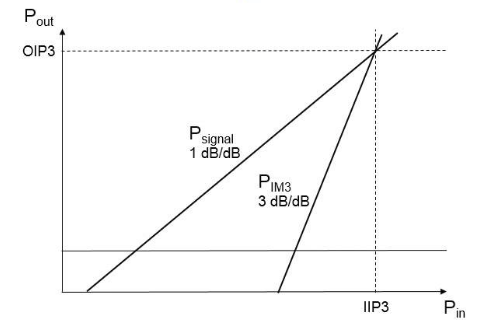
\includegraphics[scale = 0.7]{pic/IP3.png}\\ \end{center}
    Ainsi nous pouvons élaborer une statégie pour mesurer le point d'IP3 experimentalement :
Il suffit d'augmenter la puissance d'entrée, tout en mesurant la sortie a l'analyseur de spectre.
Dès que les puissances d'IM3 et du premier ton sont au meme niveau, on peut être sûr qu'on est sur le point d'IP3.
\chapter{Conclusion}

    Pour conclure ce TP, nous pouvons dire que même si le mixer génère de nombreuses fréquences parasites, 
il reste très utile pour traiter le signal radio entrant. De plus, lorsqu'on regarde le spectre en mW, et non plus
en dBm, il apparait de façon flagrante que les fréquences parasites sont bien en dessous des fréquences
réèlement utilisés, comme nous pouvons le voir sur le graphique ci-dessous. 
\begin{center}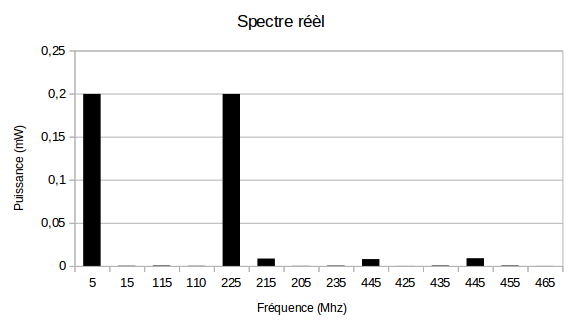
\includegraphics[scale = 0.7]{pic/spectre_mw.png}\\ \end{center}
Cependant il sera quand même préférable d'utiliser un filtre pour eviter toute surprise.
\chapter{Annexe}
Voici quelques relevés obtenue lors des tests
\begin{center}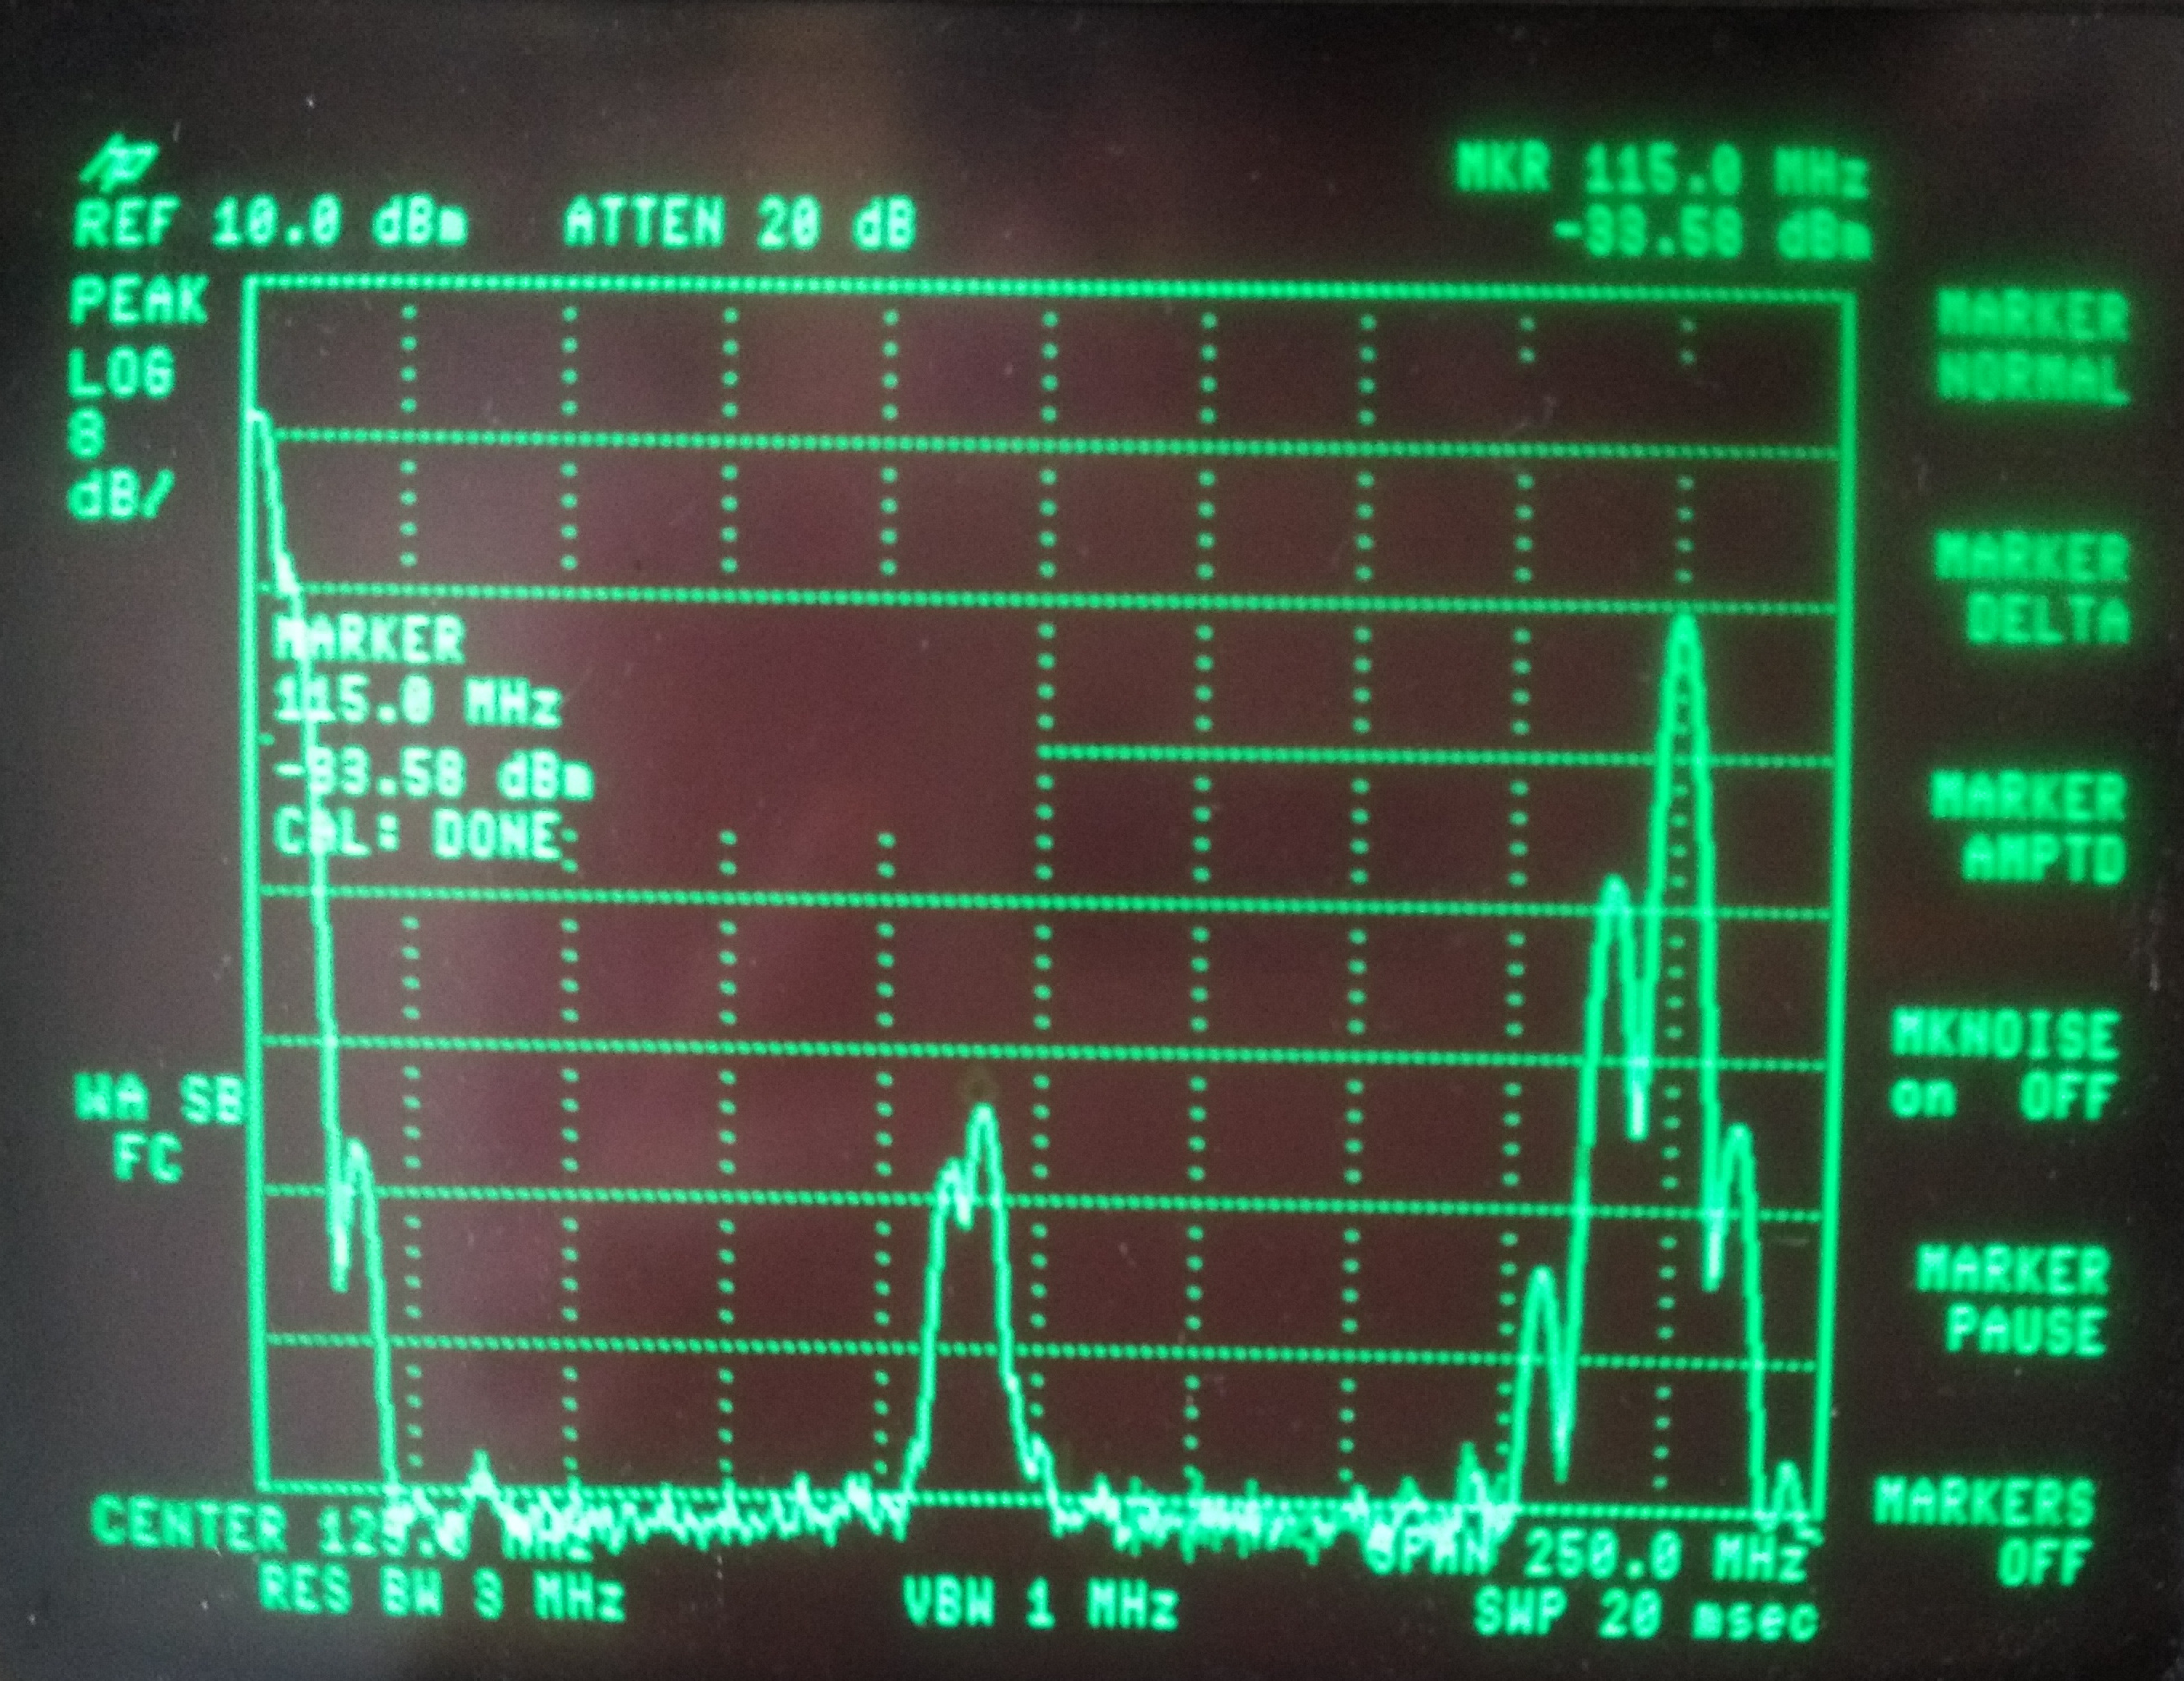
\includegraphics[scale = 0.1]{pic/photo2.jpg}\\ \end{center}
    Première phase de test, spectre faisant apparaitre les raies OL-RF et OL+RF,
    ainsi que OL et RF.
\begin{center}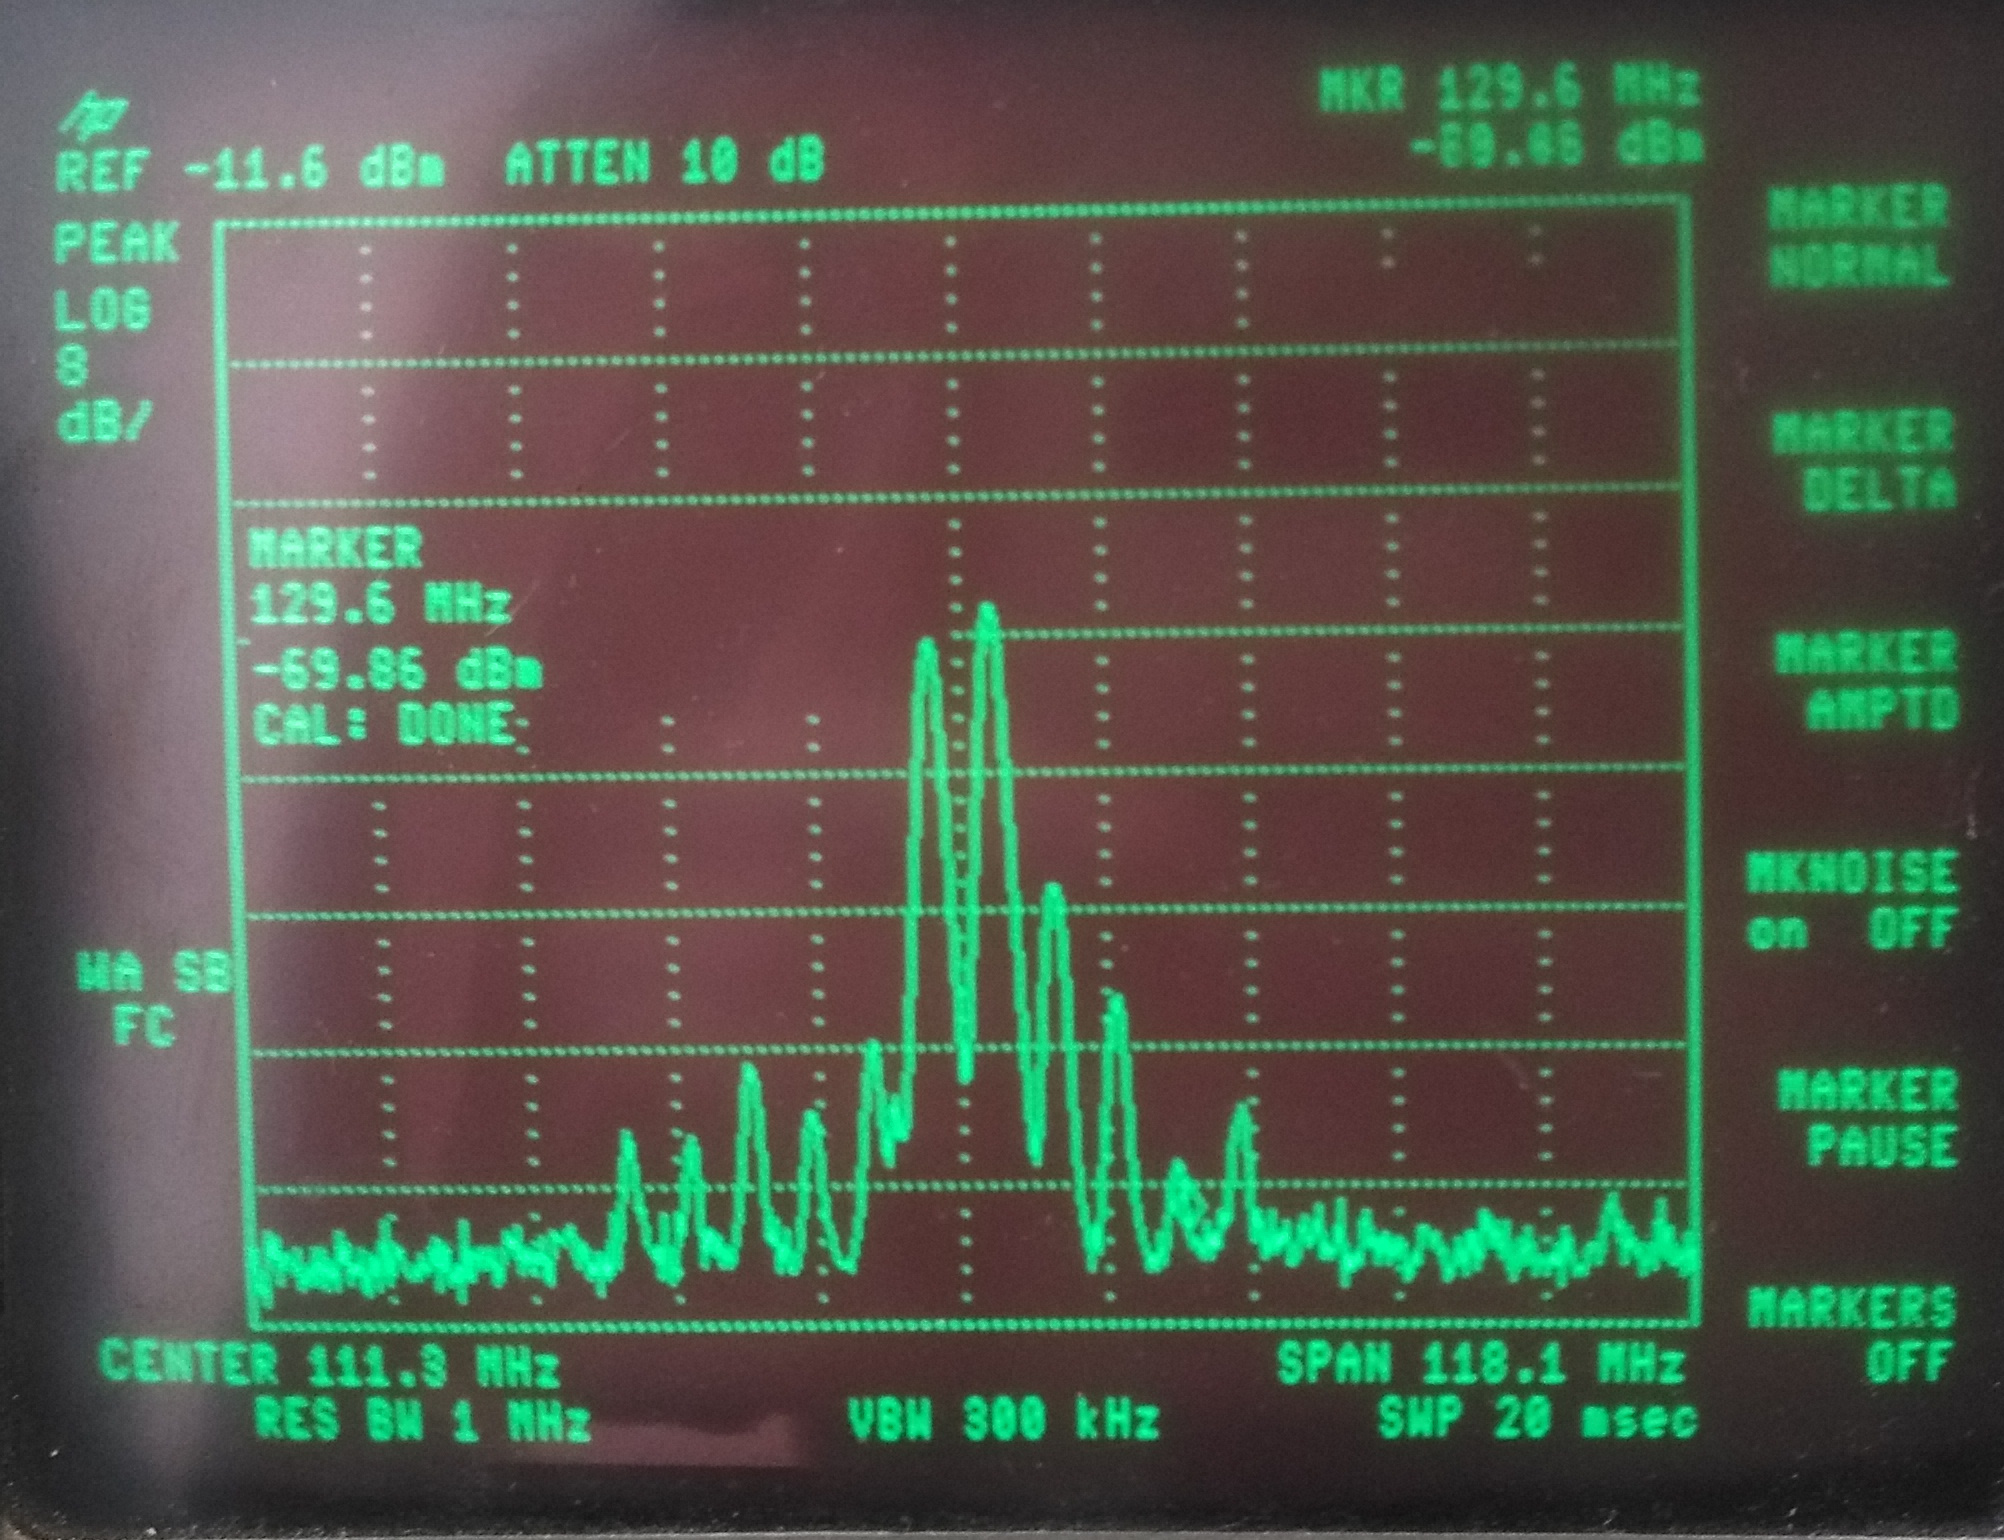
\includegraphics[scale = 0.14]{pic/photo3.jpg}\\ \end{center}
    Zoom établie sur les raies OL et RF.
\begin{center}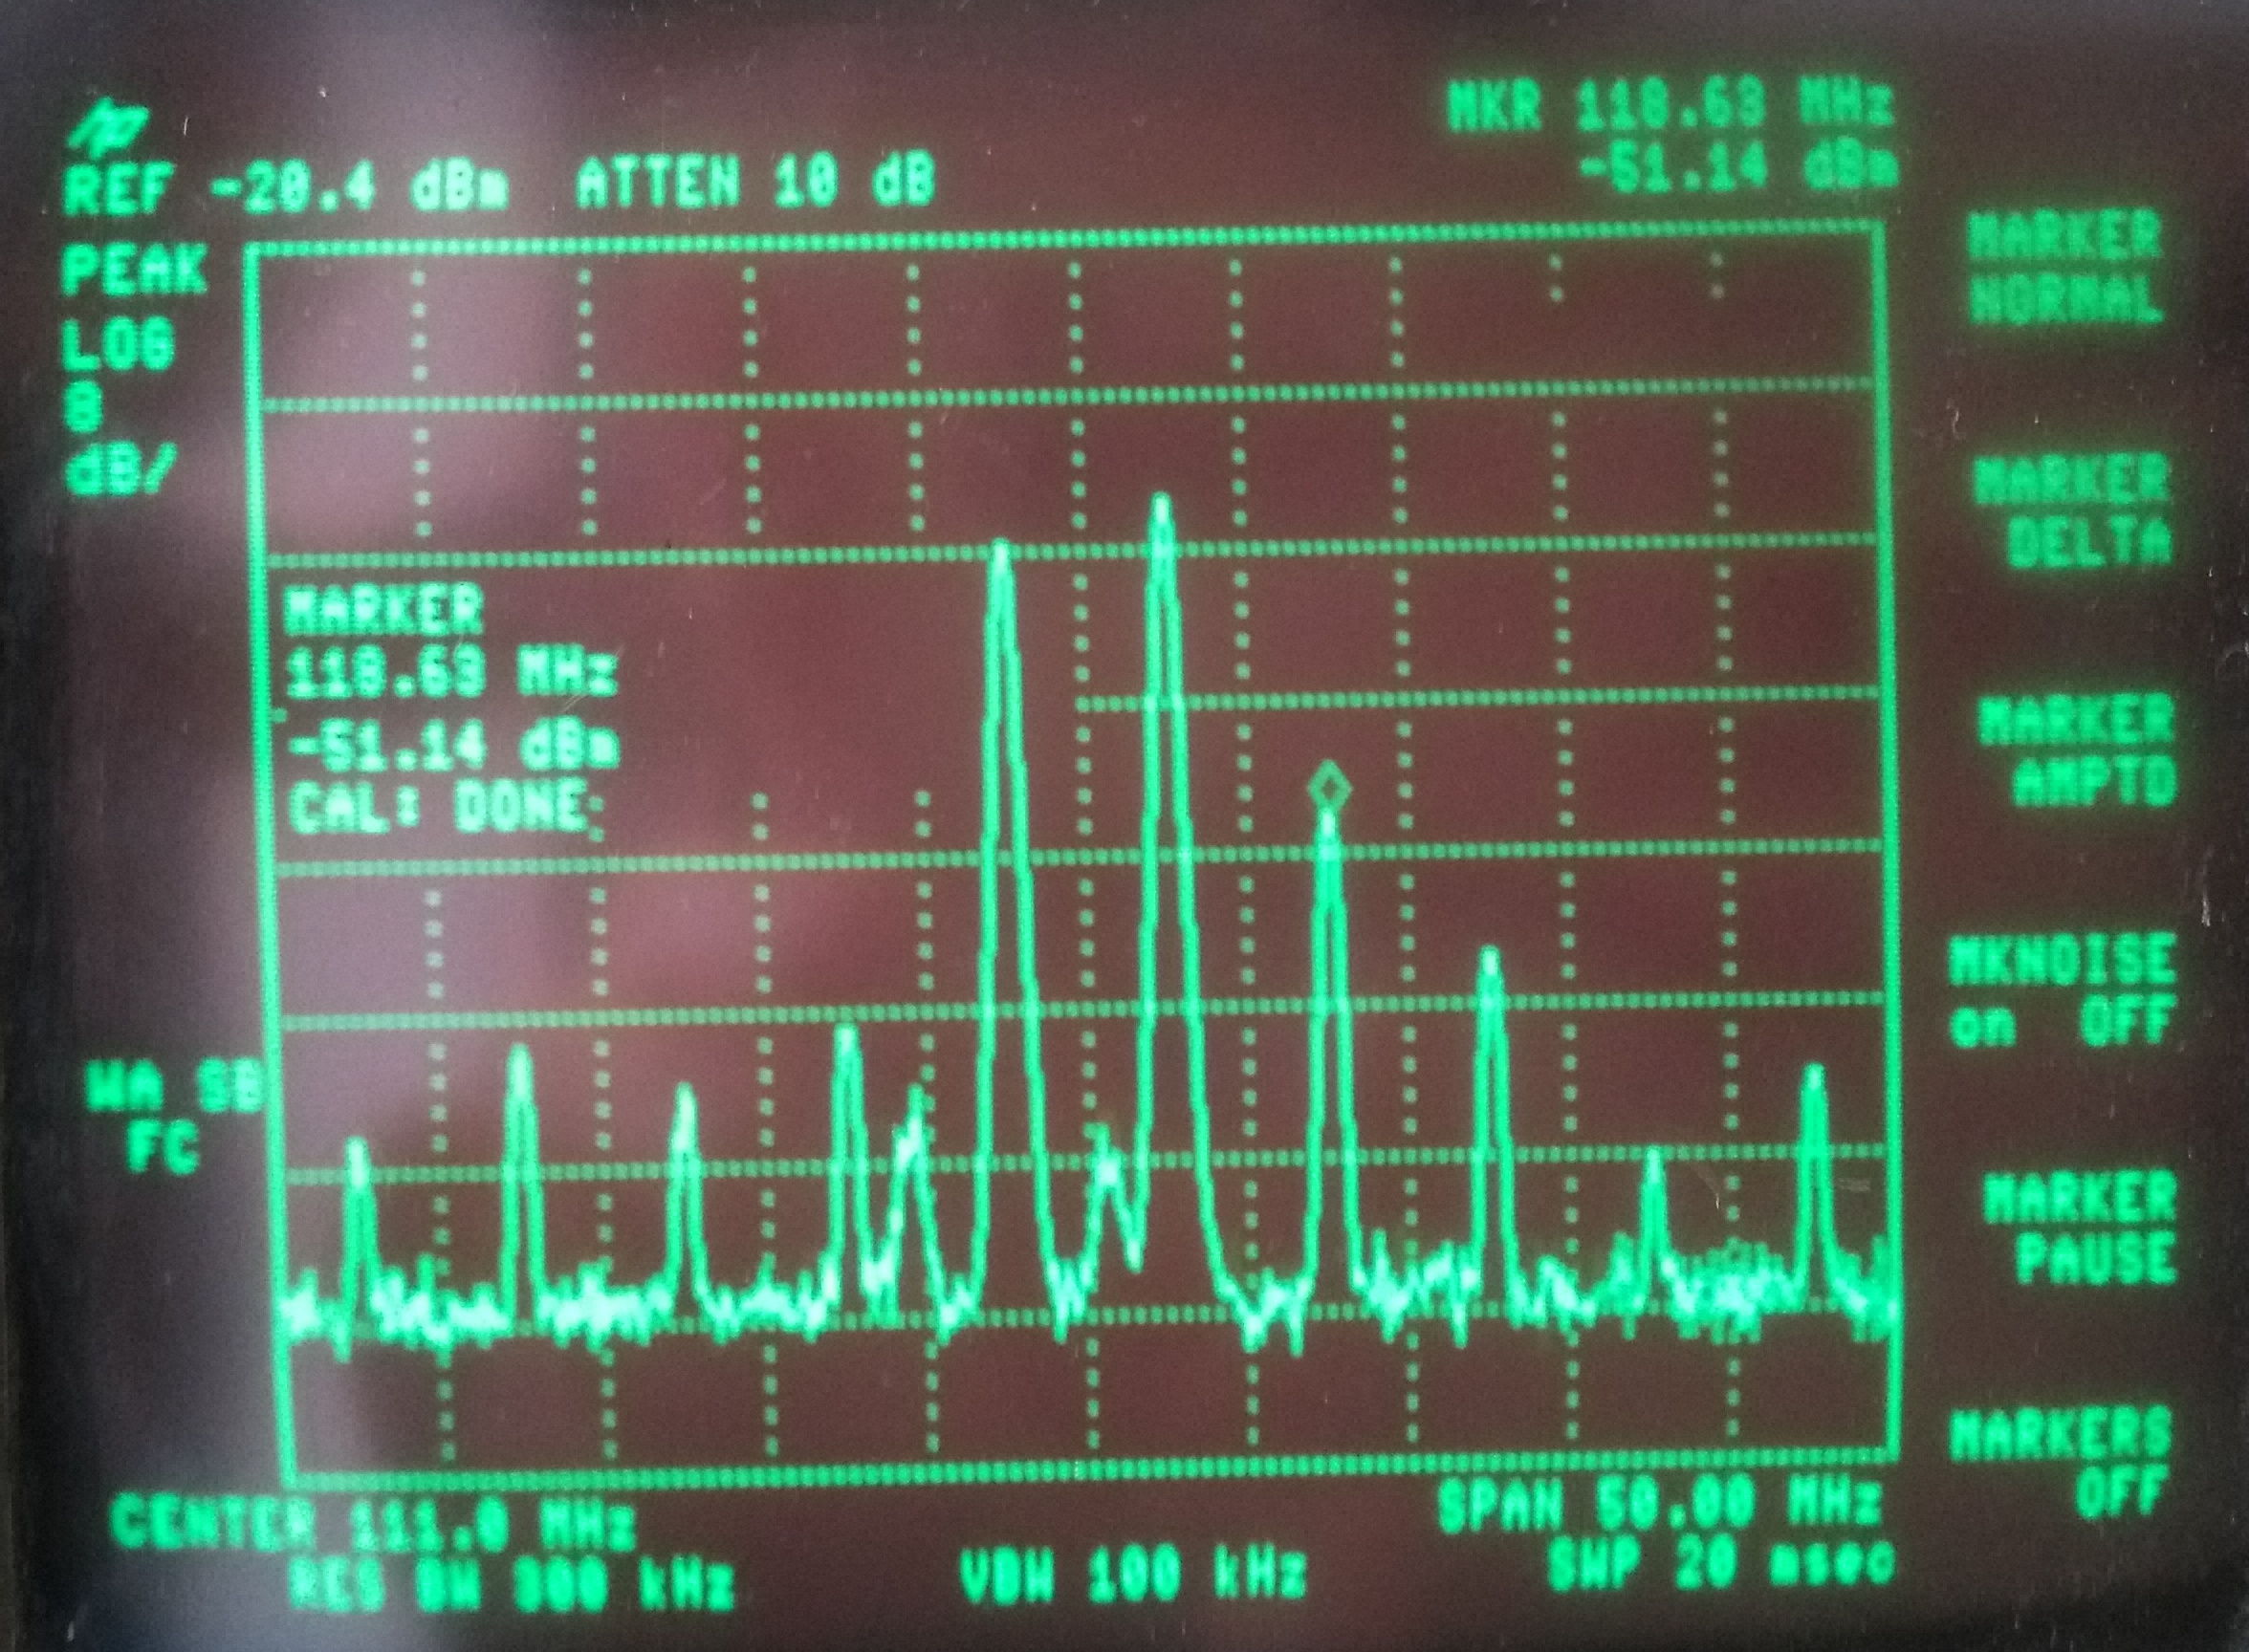
\includegraphics[scale = 0.12]{pic/photo4.jpg}\\ \end{center}
    Même spectre que précédement avec une précision plus importante.
\begin{center}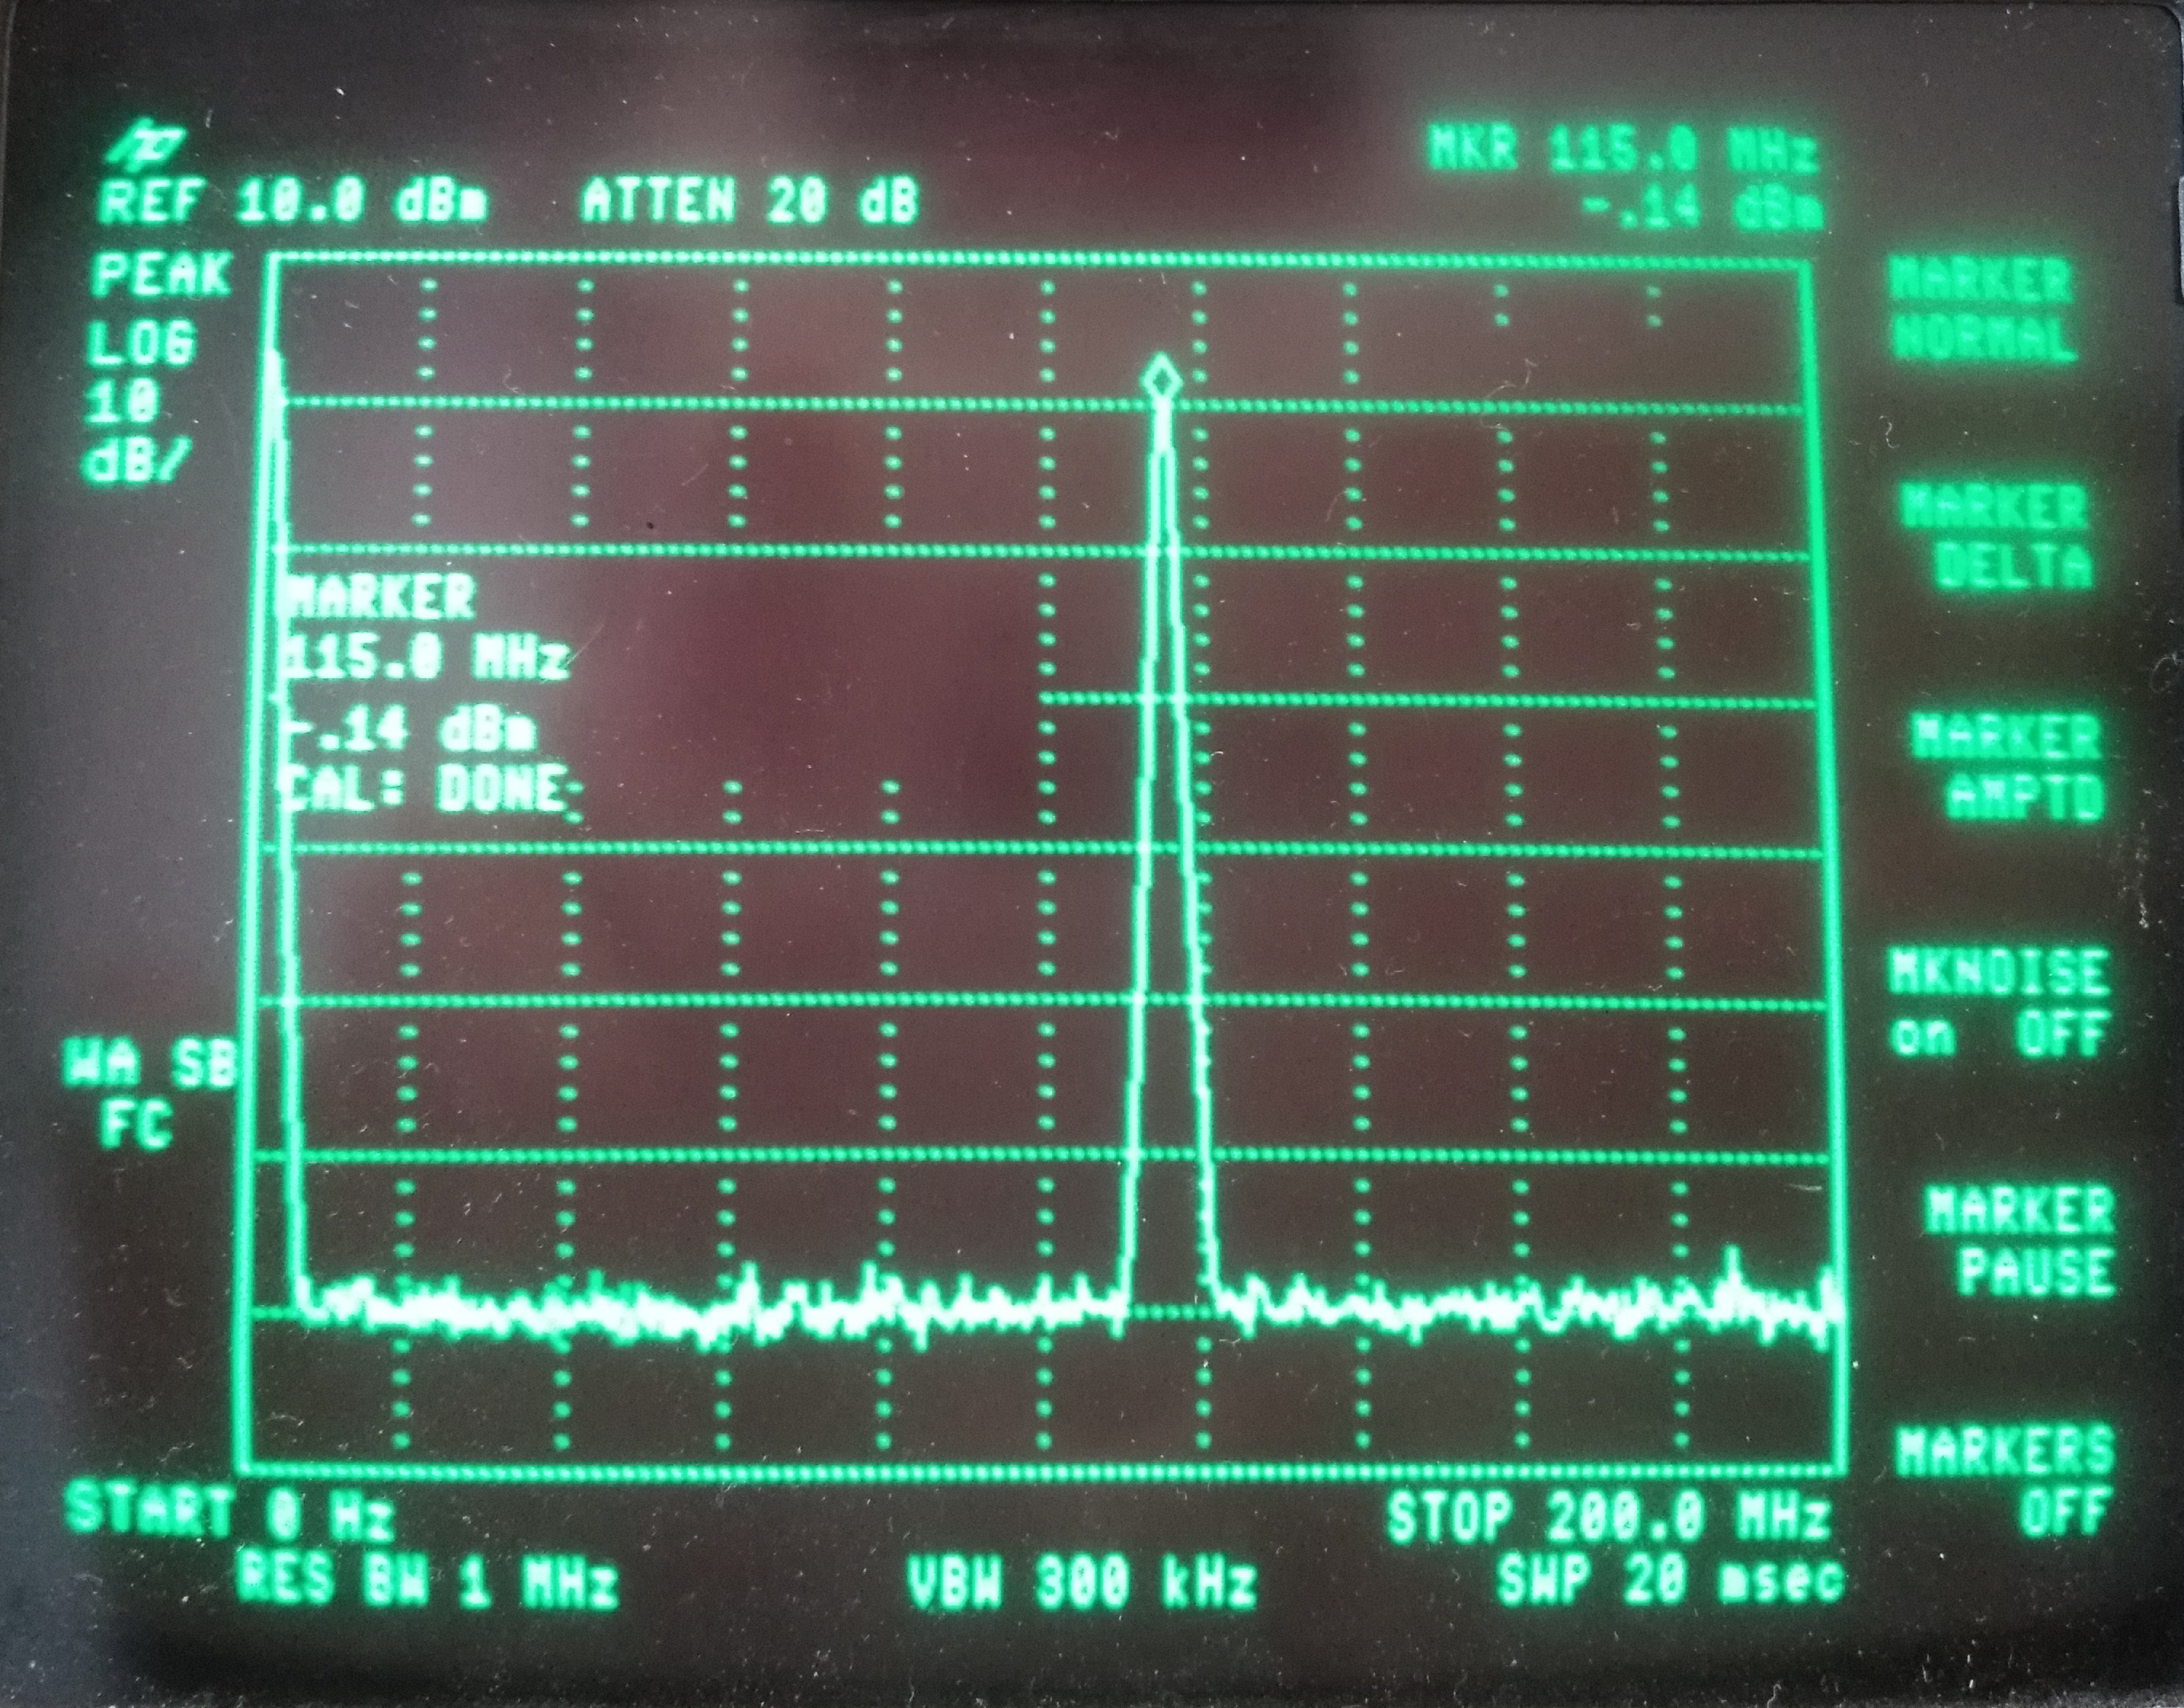
\includegraphics[scale = 0.11]{pic/photo1.jpg}\\ \end{center}
    visualisation du spectre RF seul.
\addcontentsline{toc}{chapter}{Conclusion}
\end{document}

